% \LaTeX-Main\
%% The LaTeX package tcolorbox - version 5.1.1 (2022/06/24)
%% tcolorbox-tutorial-poster.tex: a tutorial for poster creation with tcolorbox
%%
%% -------------------------------------------------------------------------------------------
%% Copyright (c) 2006-2022 by Prof. Dr. Dr. Thomas F. Sturm <thomas dot sturm at unibw dot de>
%% -------------------------------------------------------------------------------------------
%%
%% This work may be distributed and/or modified under the
%% conditions of the LaTeX Project Public License, either version 1.3
%% of this license or (at your option) any later version.
%% The latest version of this license is in
%%   http://www.latex-project.org/lppl.txt
%% and version 1.3 or later is part of all distributions of LaTeX
%% version 2005/12/01 or later.
%%
%% This work has the LPPL maintenance status `author-maintained'.
%%
%% This work consists of all files listed in README
%%
% arara: pdflatex: { shell: yes }
% arara: pdflatex: { shell: yes }
\documentclass[36pt]{article}

%\usepackage[a0paper,landscape]{geometry}
\usepackage[paperwidth=180cm,paperheight=120cm]{geometry}
\usepackage{layout}
\usepackage{lipsum}
\usepackage{lmodern}
\usepackage{enumerate}
\usepackage[poster]{tcolorbox}
\usepackage[round]{natbib}
\usepackage{hyperref}
\usepackage{multicol}
\renewcommand{\bibsection}{} % works with natbib get rid of the Reference in the bibliography (We already have it in the title of the box
\tcbuselibrary{minted} % <- replace by \tcbuselibrary{listings}, if minted does not work for you

\pagestyle{empty}


%\usepackage{authblk}
%\title{This is some thing}
%\author[1]{Don Joe}
%\author[2]{Smith K.}
%\author[1]{Wanderer}
%\author[1]{Static}
%\affil[1]{TeX.SX}
%\affil[2]{Both on a bus}
%\setcounter{Maxaffil}{0}
%\renewcommand\Affilfont{\itshape\small}

\begin{document}
\begin{tcbposter}[
  coverage = {
      spread,
      interior style={top color=white,bottom color=white!50!red},
      watermark text={Cornell University CALS},
      watermark color=white,
      %toptitle=25mm,
      %bottomtitle=25mm,
  },
  poster   = {
    %showframe,
    spacing=1cm,
    %colspacing=1cm,
    %rowspacing=1cm,
    columns=4,
    rows=5
  },
  fontsize = 32pt,
  boxes = {
    enhanced standard jigsaw,sharp corners=downhill,arc=12mm,boxrule=4mm,
    colback=white,opacityback=0.75,colframe=white,
    title style={left color=black,right color=red},
    %fonttitle=\bfseries\Huge\scshape,
    fonttitle=\bfseries\Large\scshape,
    left=1cm,
    right=1cm
  },
]

%----
\posterbox[blankest,interior engine=path,height=11cm,
halign=center,valign=center,fontupper=\bfseries\large,colupper=red!25!black,
underlay={
\node[right,inner sep=0pt,outer sep=0pt] at (frame.west) {
\includegraphics[height=11cm]{bold_cornell_seal_print/bold_cornell_seal_cmyk_red.pdf}};
\node[left,inner sep=0pt,outer sep=0pt] at (frame.east) {
\includegraphics[height=11cm]{Vertical-Wordmark-red.pdf}};
},
]{
name=title,
column=1,
span=4,
below=top}{
\resizebox*{!}{2cm}
%\resizebox{90cm}{!}
{ \bfseries Reproducible Carbon Cycle Models bgc\_md2 }\\[6mm]
{ \bfseries Open Source Biogeochemical Model Database}\\[6mm]
\begin{minipage}{150cm}
\begin{center}
\small{
%\maketitle
Markus Müller $^1$, 
Holger Metzler $^2$,
% Verónika Ceballos Núñez3,
Ver\'onika Ceballos-N\'u\~nez $^3$
Kostiantyn Viatkin $^1$,
Jon Wells $^5$,
Yu Zhou $^1$,
Cuijuan Liao $^6$,
Aneesh Chandel$^1$,
Feng Tao $^6$,
Yuanyuan Huang $^7$,
Alison Bennett $^8$,
Song Wang $^9$,
Chenyu Bian $^{10}$,
Chengcheng Gang $^{11}$,
{Lifen Jiang $^{5}$},
Carlos A Sierra $^{13}$ and Yiqi Luo $^1$
}
\end{center}
\tiny{ 
(1) Cornell University, 
%School of Integrative Plant Science, 
Ithaca, United States, 
(2) Swedish University of Agricultural Sciences, 
%Department of Crop Production Ecology, 
Uppsala, Sweden, 
(3) Leipzig University, 
%German Centre for Integrative Biodiversity Research (iDiv), 
%Halle-Jena-Leipzig, 
Germany, 
(5) Northern Arizona University, 
%Center for Ecosystem Sciences and Society, 
Flagstaff, United States, 
(6) Tsinghua University, Department of Earth System Science, Beijing, China, 
(7) LSCE Laboratoire des Sciences du Climat et de l'Environnement, 
Gif-Sur-Yvette Cedex, France, 
(8) University of Melbourne, 
%School of Ecosystem and Forest Science, 
%Parkville, VIC, Australia, 
(9) IGSNRR Institute of Geographic Sciences and Natural Resources Research, CAS, 
%Key Laboratory of Ecosystem Network Observation and Modeling, 
Beijing, China, 
(10) East China Normal University, School of Ecological and Environmental Sciences, Shanghai, China, 
%(11)Northwest A&F University, Institute of Soil and Water Conservation, Yangling, China, 
(13) Max Planck Institute for Biogeochemistry, 
%Theoretical Ecosystem Ecology, 
Jena, Germany
}
\end{minipage}
}


\posterbox[adjusted title=Model Creation Inspection and Querying]{
  name=overview,
  column=1,
  below=title,
  %above=bottom
  %rowspan=2,
  %below=title,
  }{
  \subsubsection*{Development}
	{ \bf bgc\_md2 } is an open source python package availabe on { \bf GitHub} , developed at the { \bf Max-Planck-Institut for BioGeoChemistry} in Jena and more recently  in Yiqi Luo's {\bf Ecolab} at NAU in Flagstaff and {\bf Cornell} in Ithaca.
	It contains collection $>$ 30 published vegetation, soil or ecosystems models as {\bf python modules}
  in a format suitable  for symbolic (\texttt{SymPy}) and numeric computations.
	It provides as set of special datatypes that describe components of the models and functions that operate on these datatypes
	and a computability graph library to {\bf compute what is computable} that can be used for queries and inspection,
  enhancing the jupyter UI to assist the creation of new models. 

\subsubsection*{Transparent Symbolic Analysis/ Numeric Computations/ Data Assimilation}
	  \begin{itemize}
	    \item 
      interactive jupiter widget with a table of models (orange buttons can be clicked to 
	    expand or collape a more detailed view of the particular model),
	    \item 
	    model inspection with pool connection graph, which can be derived from the symbolic description
	    along other symbolic properties as flux equations and the compartmental matrix,
	    \item 
      Zoom into IPython/Jupyter UI showing methods automatically added by the computability graph library. 
	    \end{itemize}
	  
    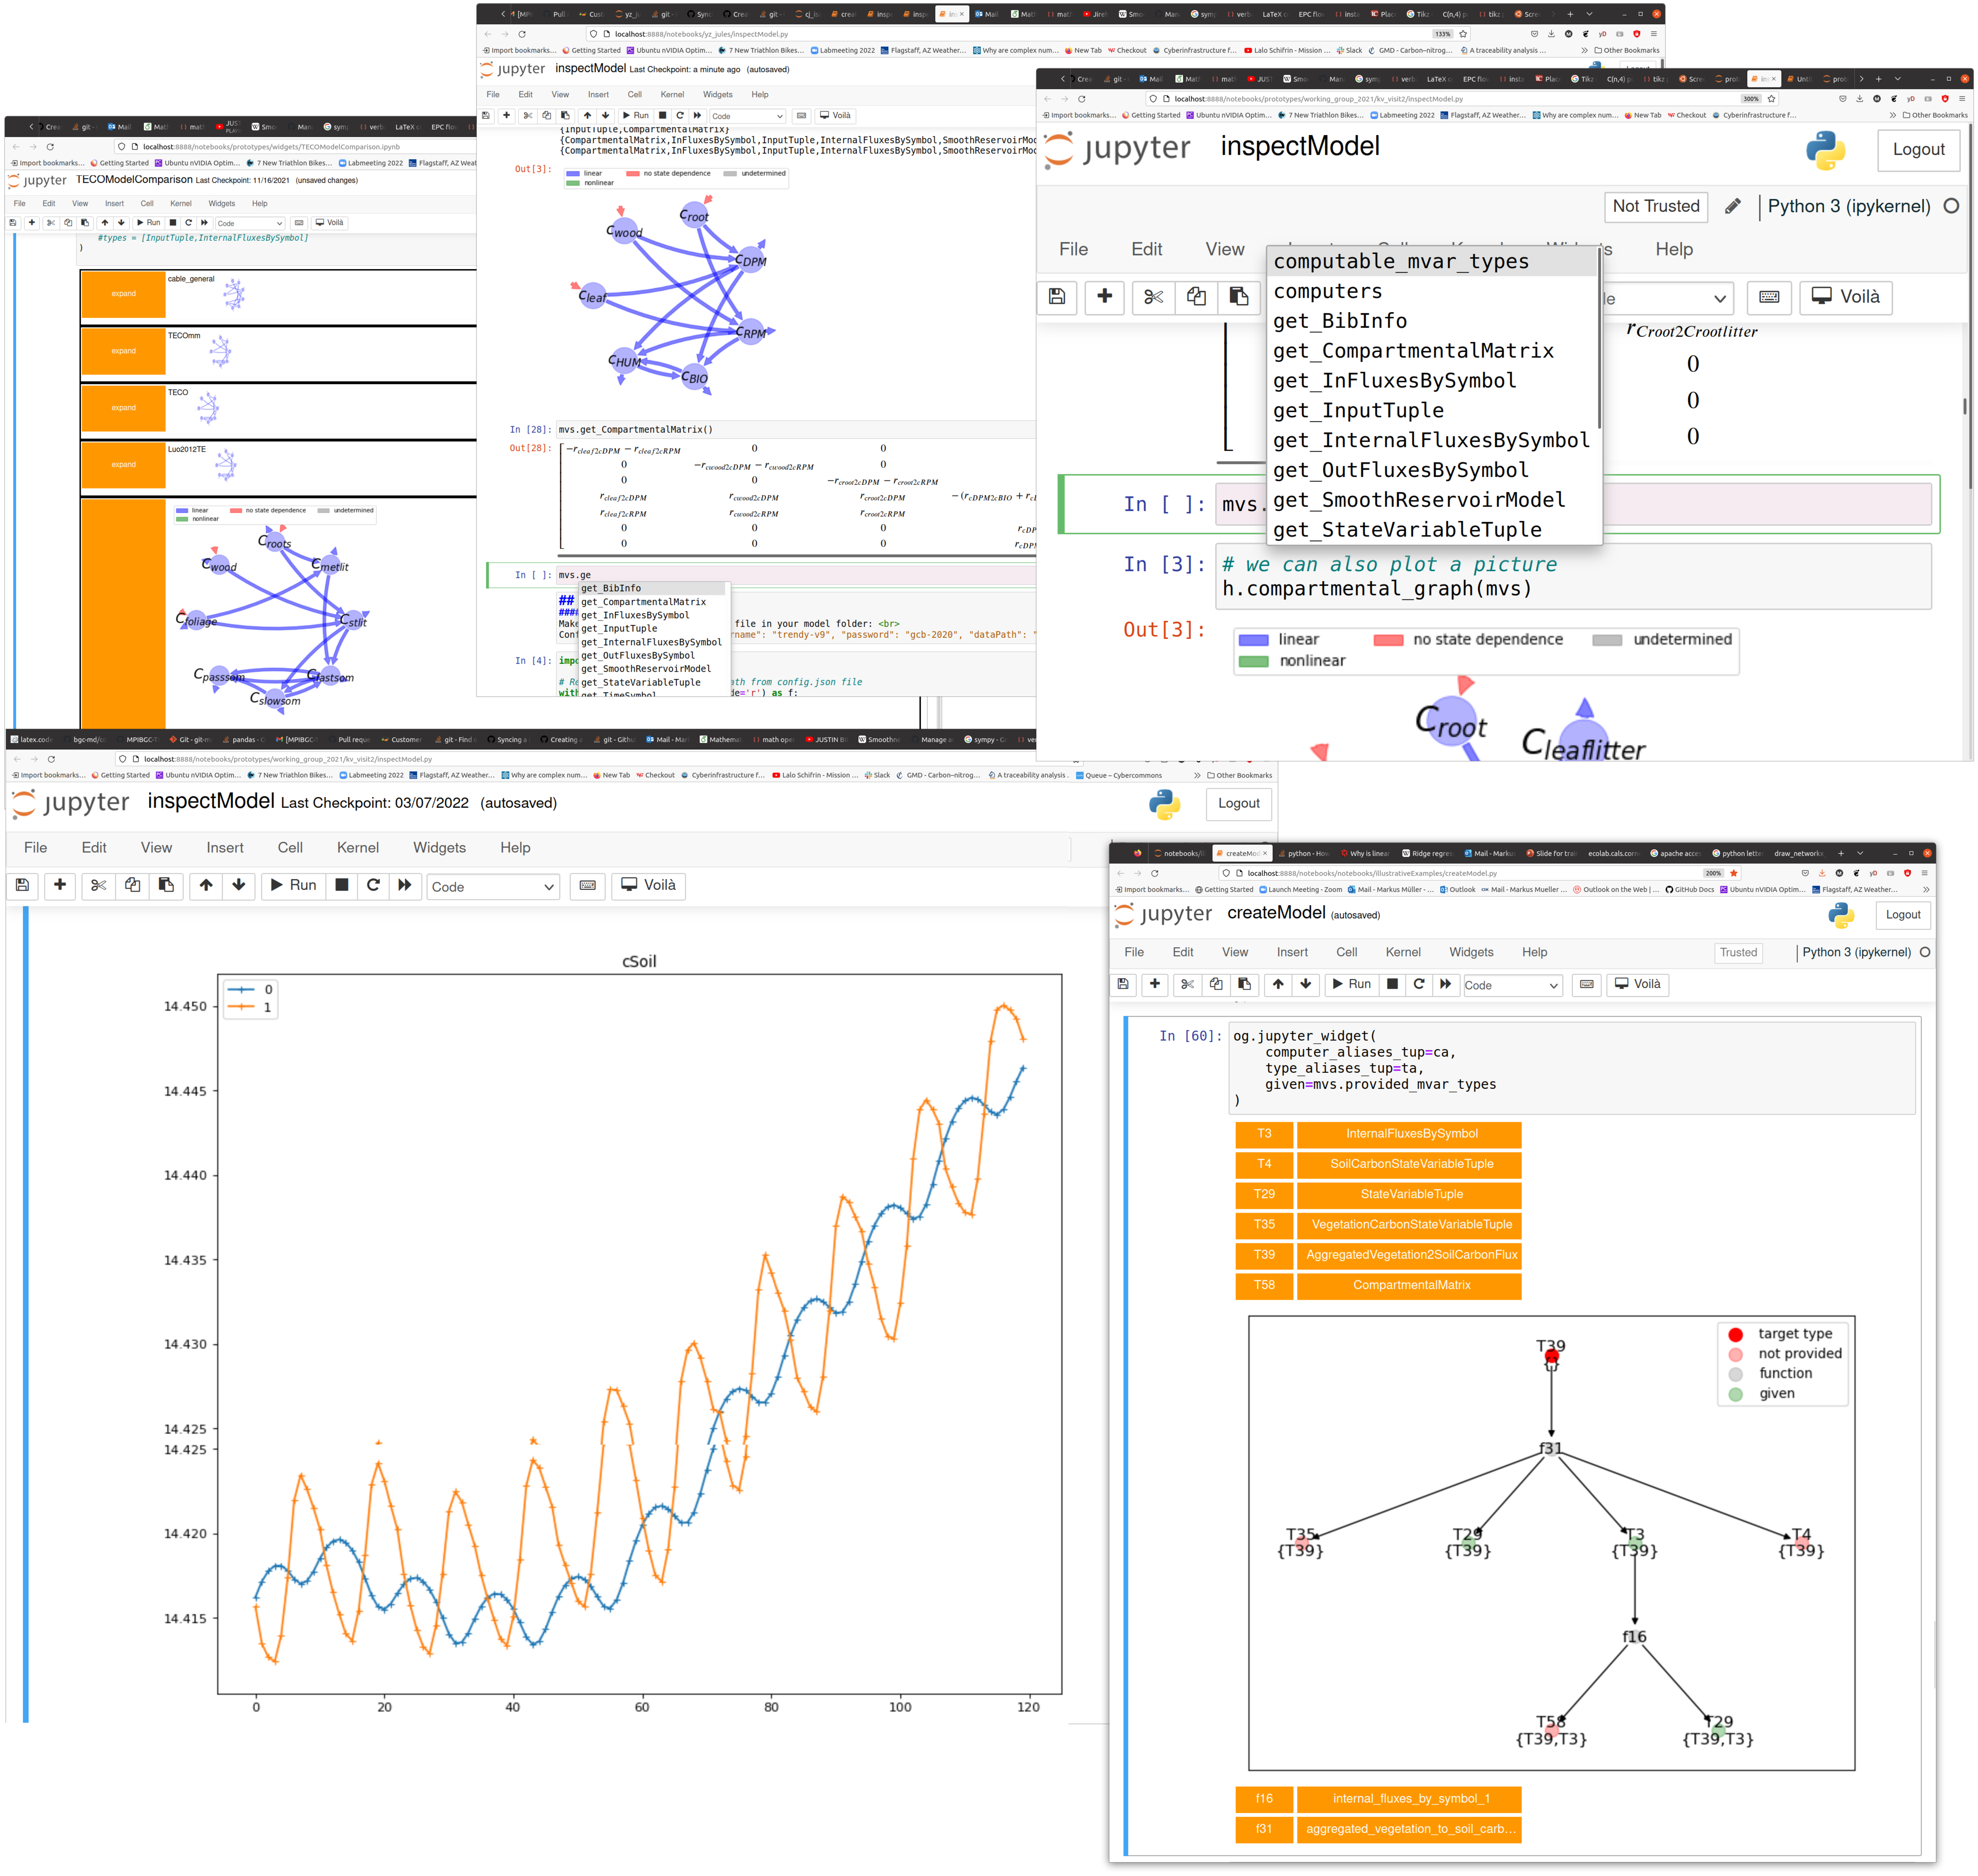
\includegraphics[width=\columnwidth]{TabScreenCombined.pdf}
	  \begin{itemize}
	    \item 
      Dataassimilation with automatically created numeric model (from symbolic description), 
	    \item 
      Computability graph for a desired diagnostic (aggregated Flux from the vegetation to soil part, showing 
      that the user has to provide more information to compute the desired result)
	  \end{itemize}
}

%%%%%%%%%%%%%%%%%%%%%%%%%%%%%%%%%%%%%%%%%%%%%%%%%%%%%%%%%%%%%%%%%%%%%%%%%%%%%%%%%%%%----
\posterbox[adjusted title=Training Course]
    {
    name=course,
    %column*=4,
    column=1,
    below=overview,
    }{
\begin{center}
	  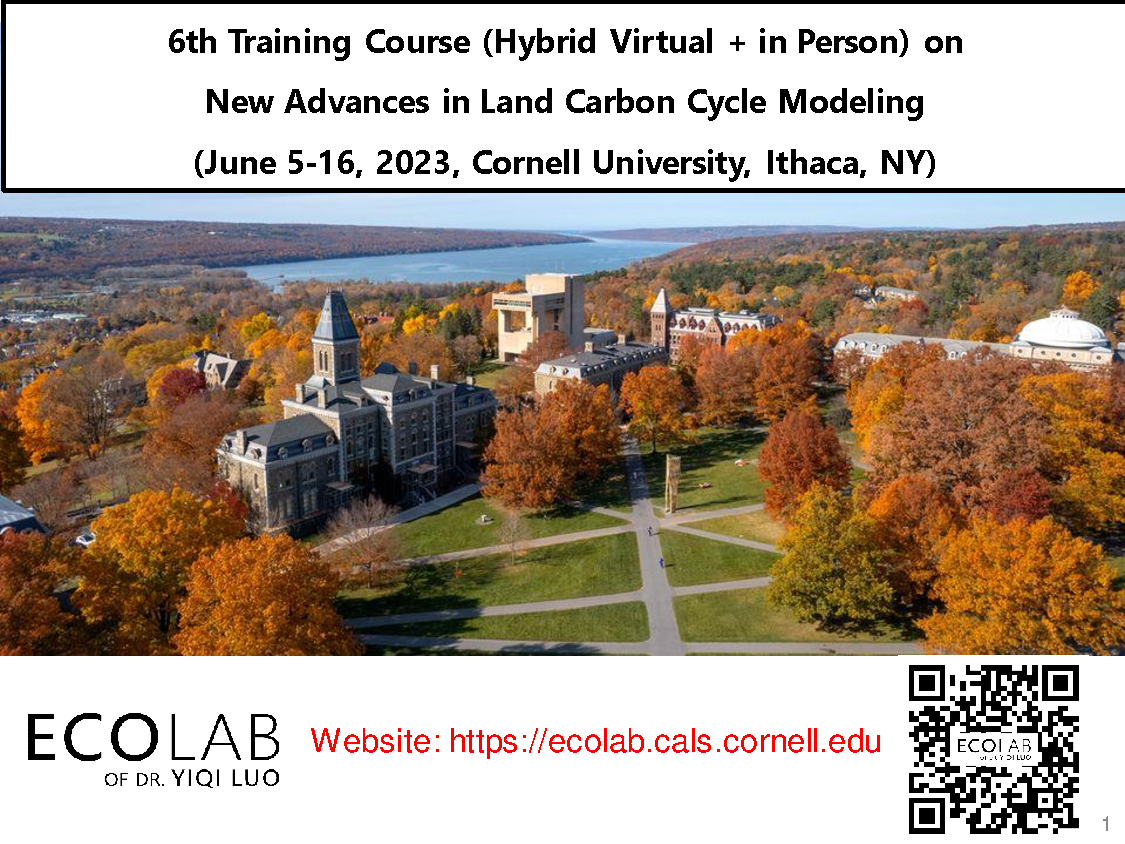
\includegraphics[width=.9\textwidth]{Slide_for_training_course.pdf}
\end{center}
}

%%%%%%%%%%%%%%%%%%%%%%%%%%%%%%%%%%%%%%%%%%%%%%%%%%%%%%%%%%%%%%%%%%%%%%%%%%%%%%%%%%%%%----
\posterbox[adjusted title=Model Inter Comparison]{
  name=ModelIntercomparison,
  column=2,
  span=2,
  below=title,
  %rowspan=2,
  %sequence=1 between overview and bottom then 2 between title and bottom
  }{
\begin{multicols}{2}
\begin{center}
  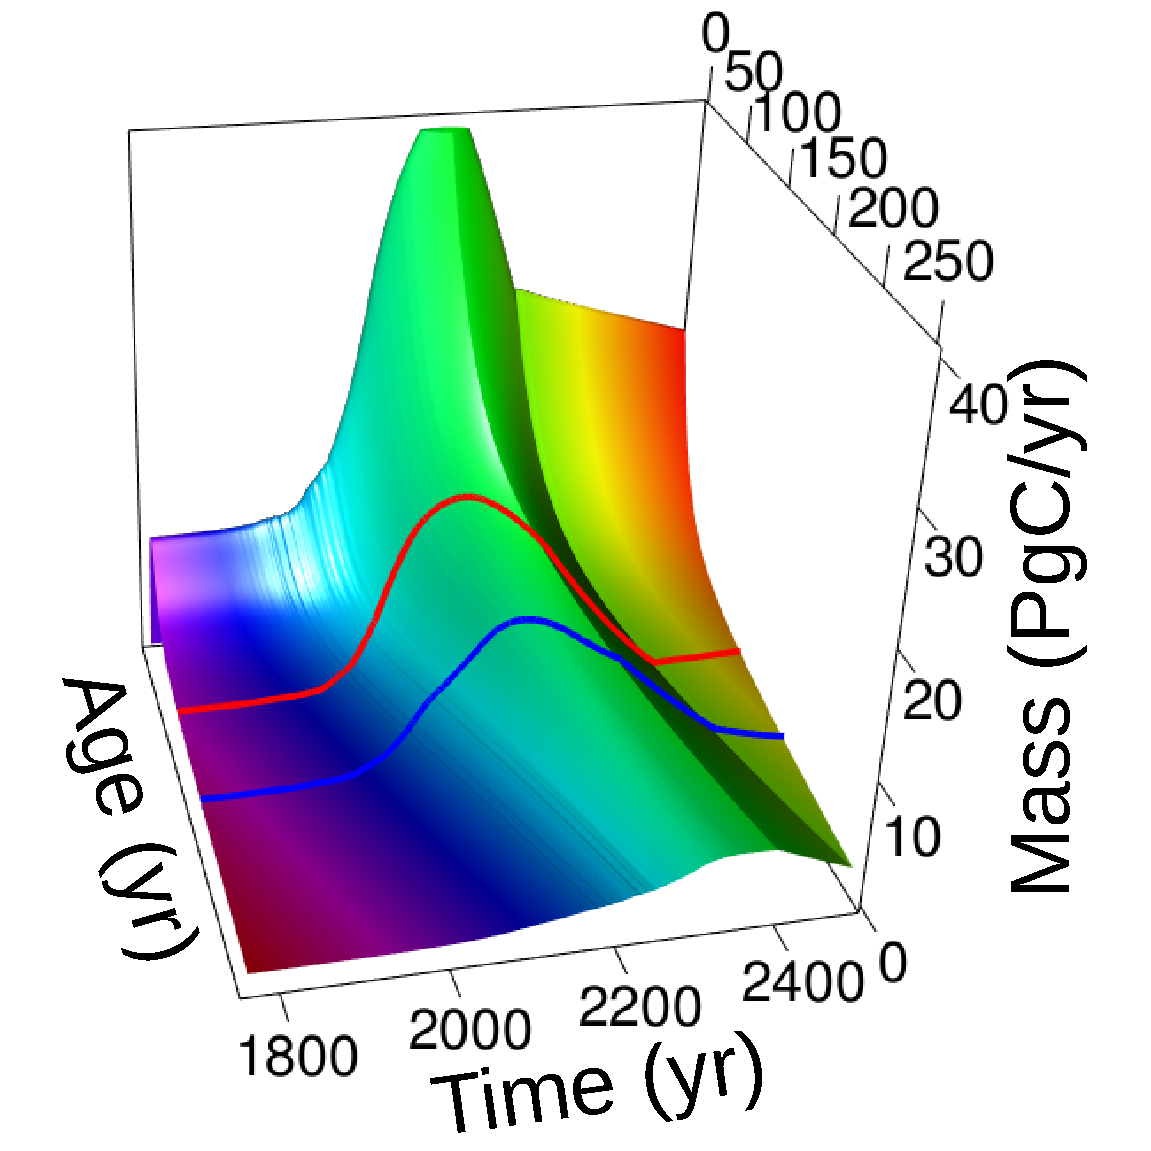
\includegraphics[width=\columnwidth]{atmosphere_nonlinear.pdf}
\end{center}
\begin{center}
	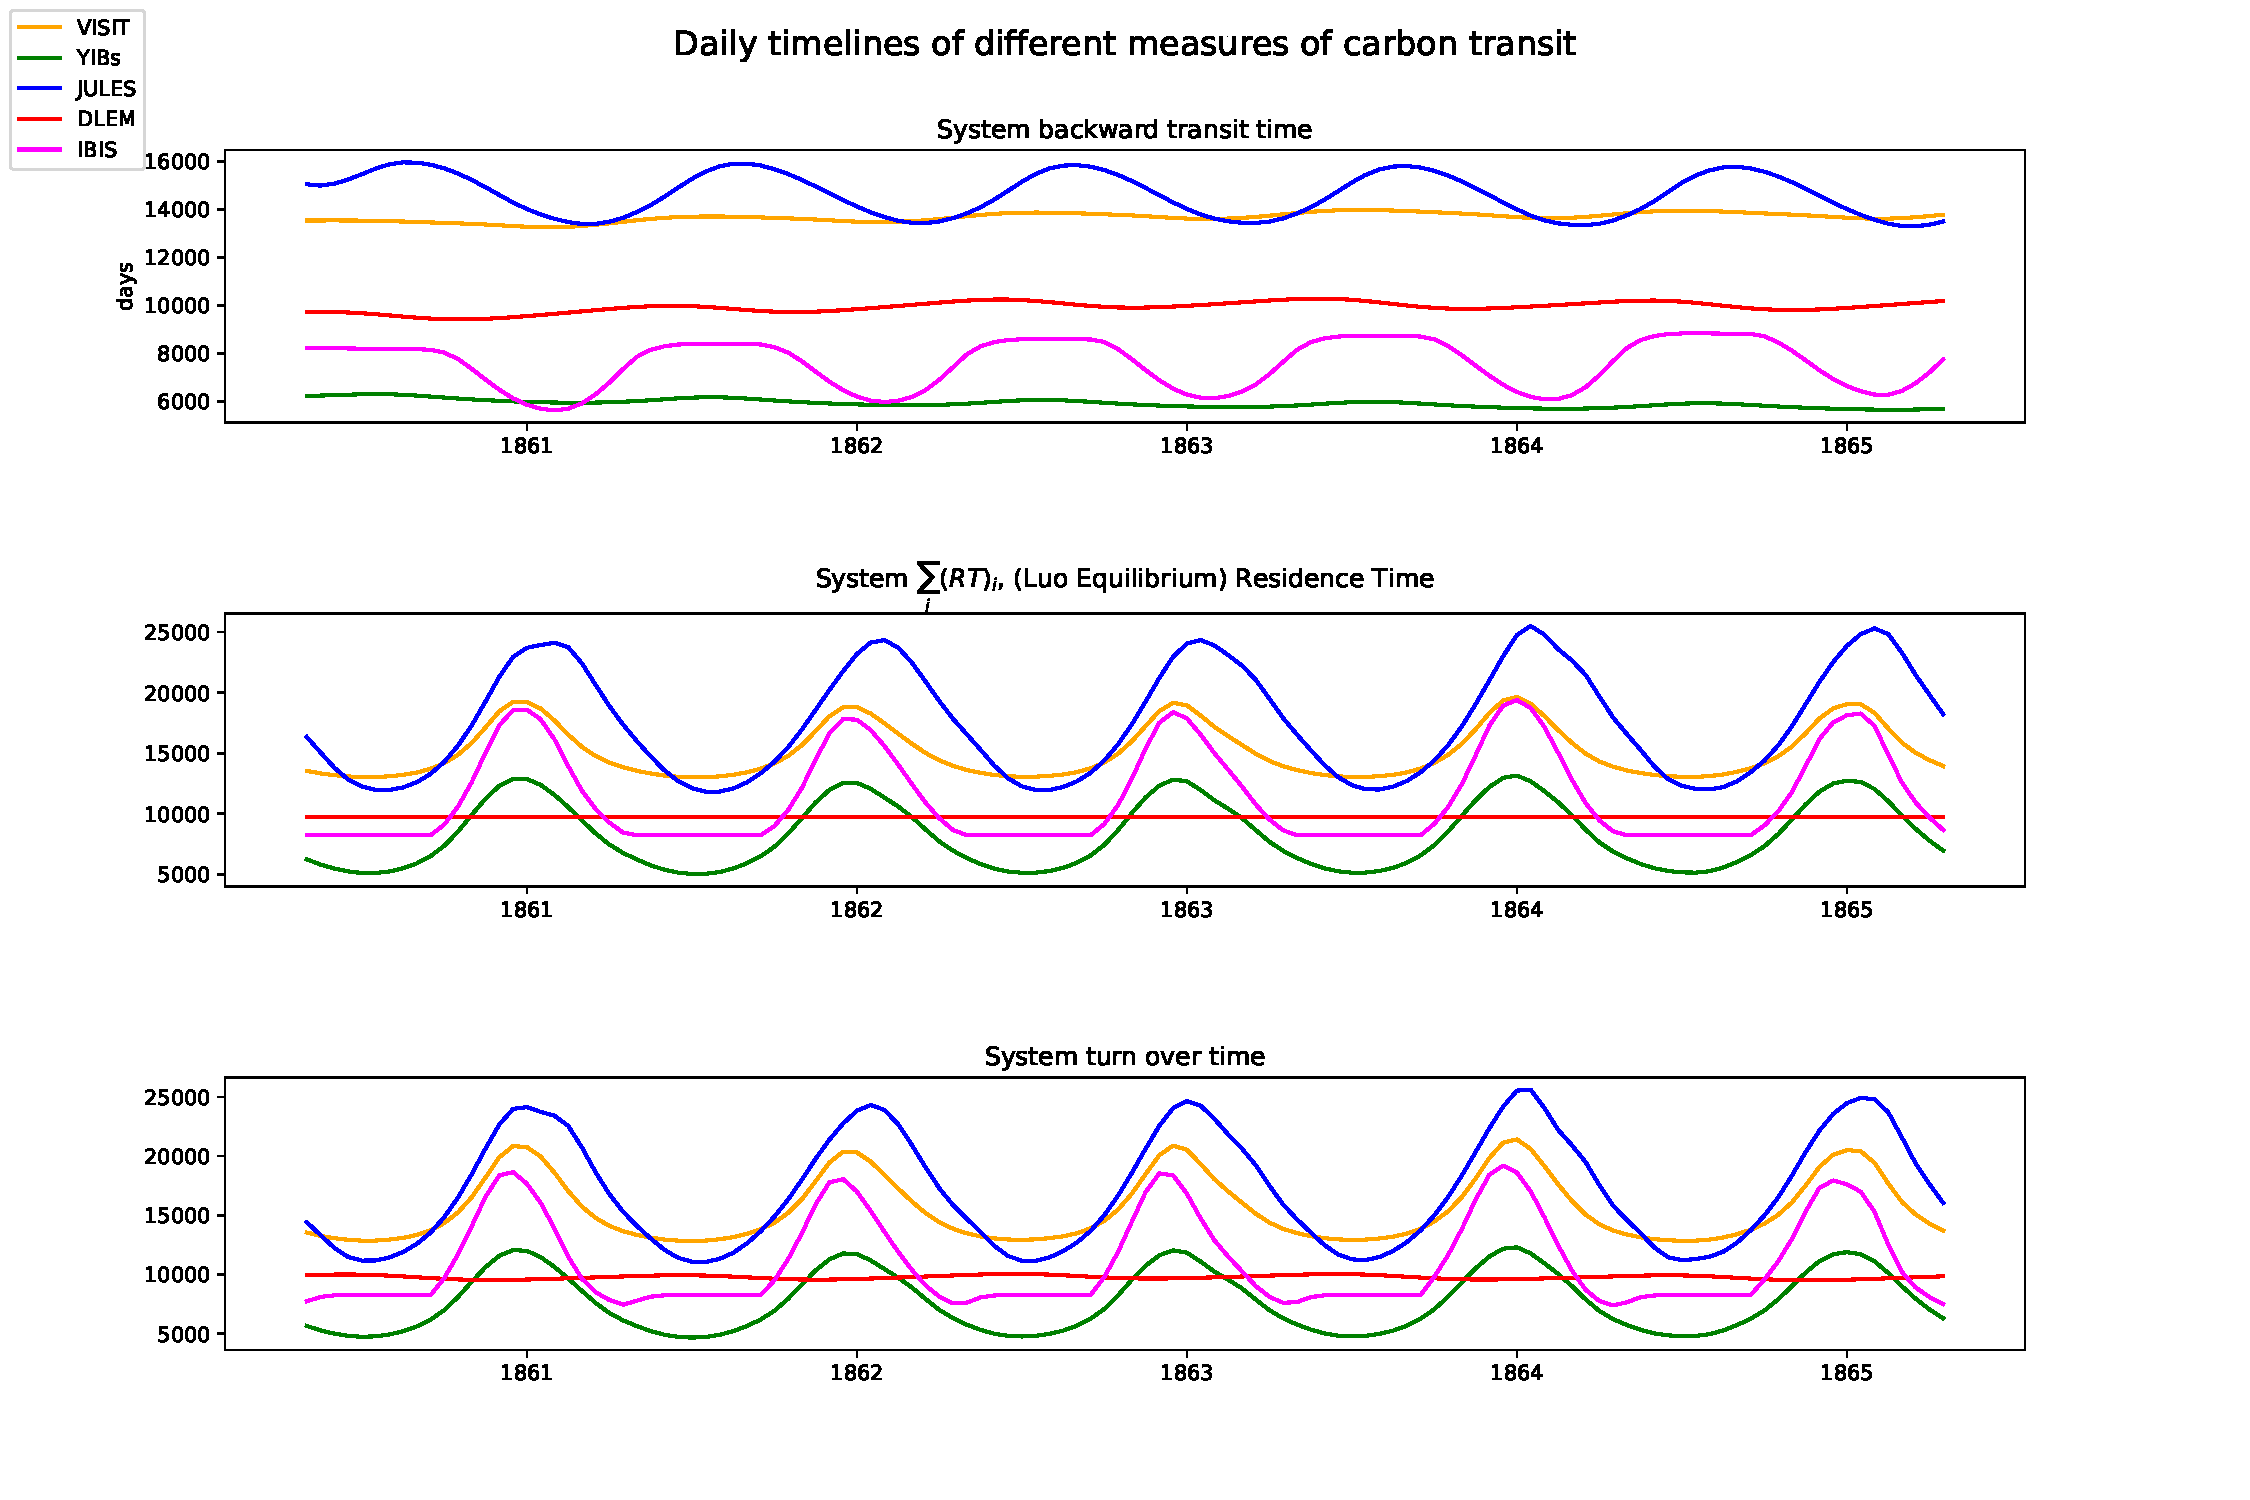
\includegraphics[width=\columnwidth]{test.pdf}
\end{center}
\begin{center}
	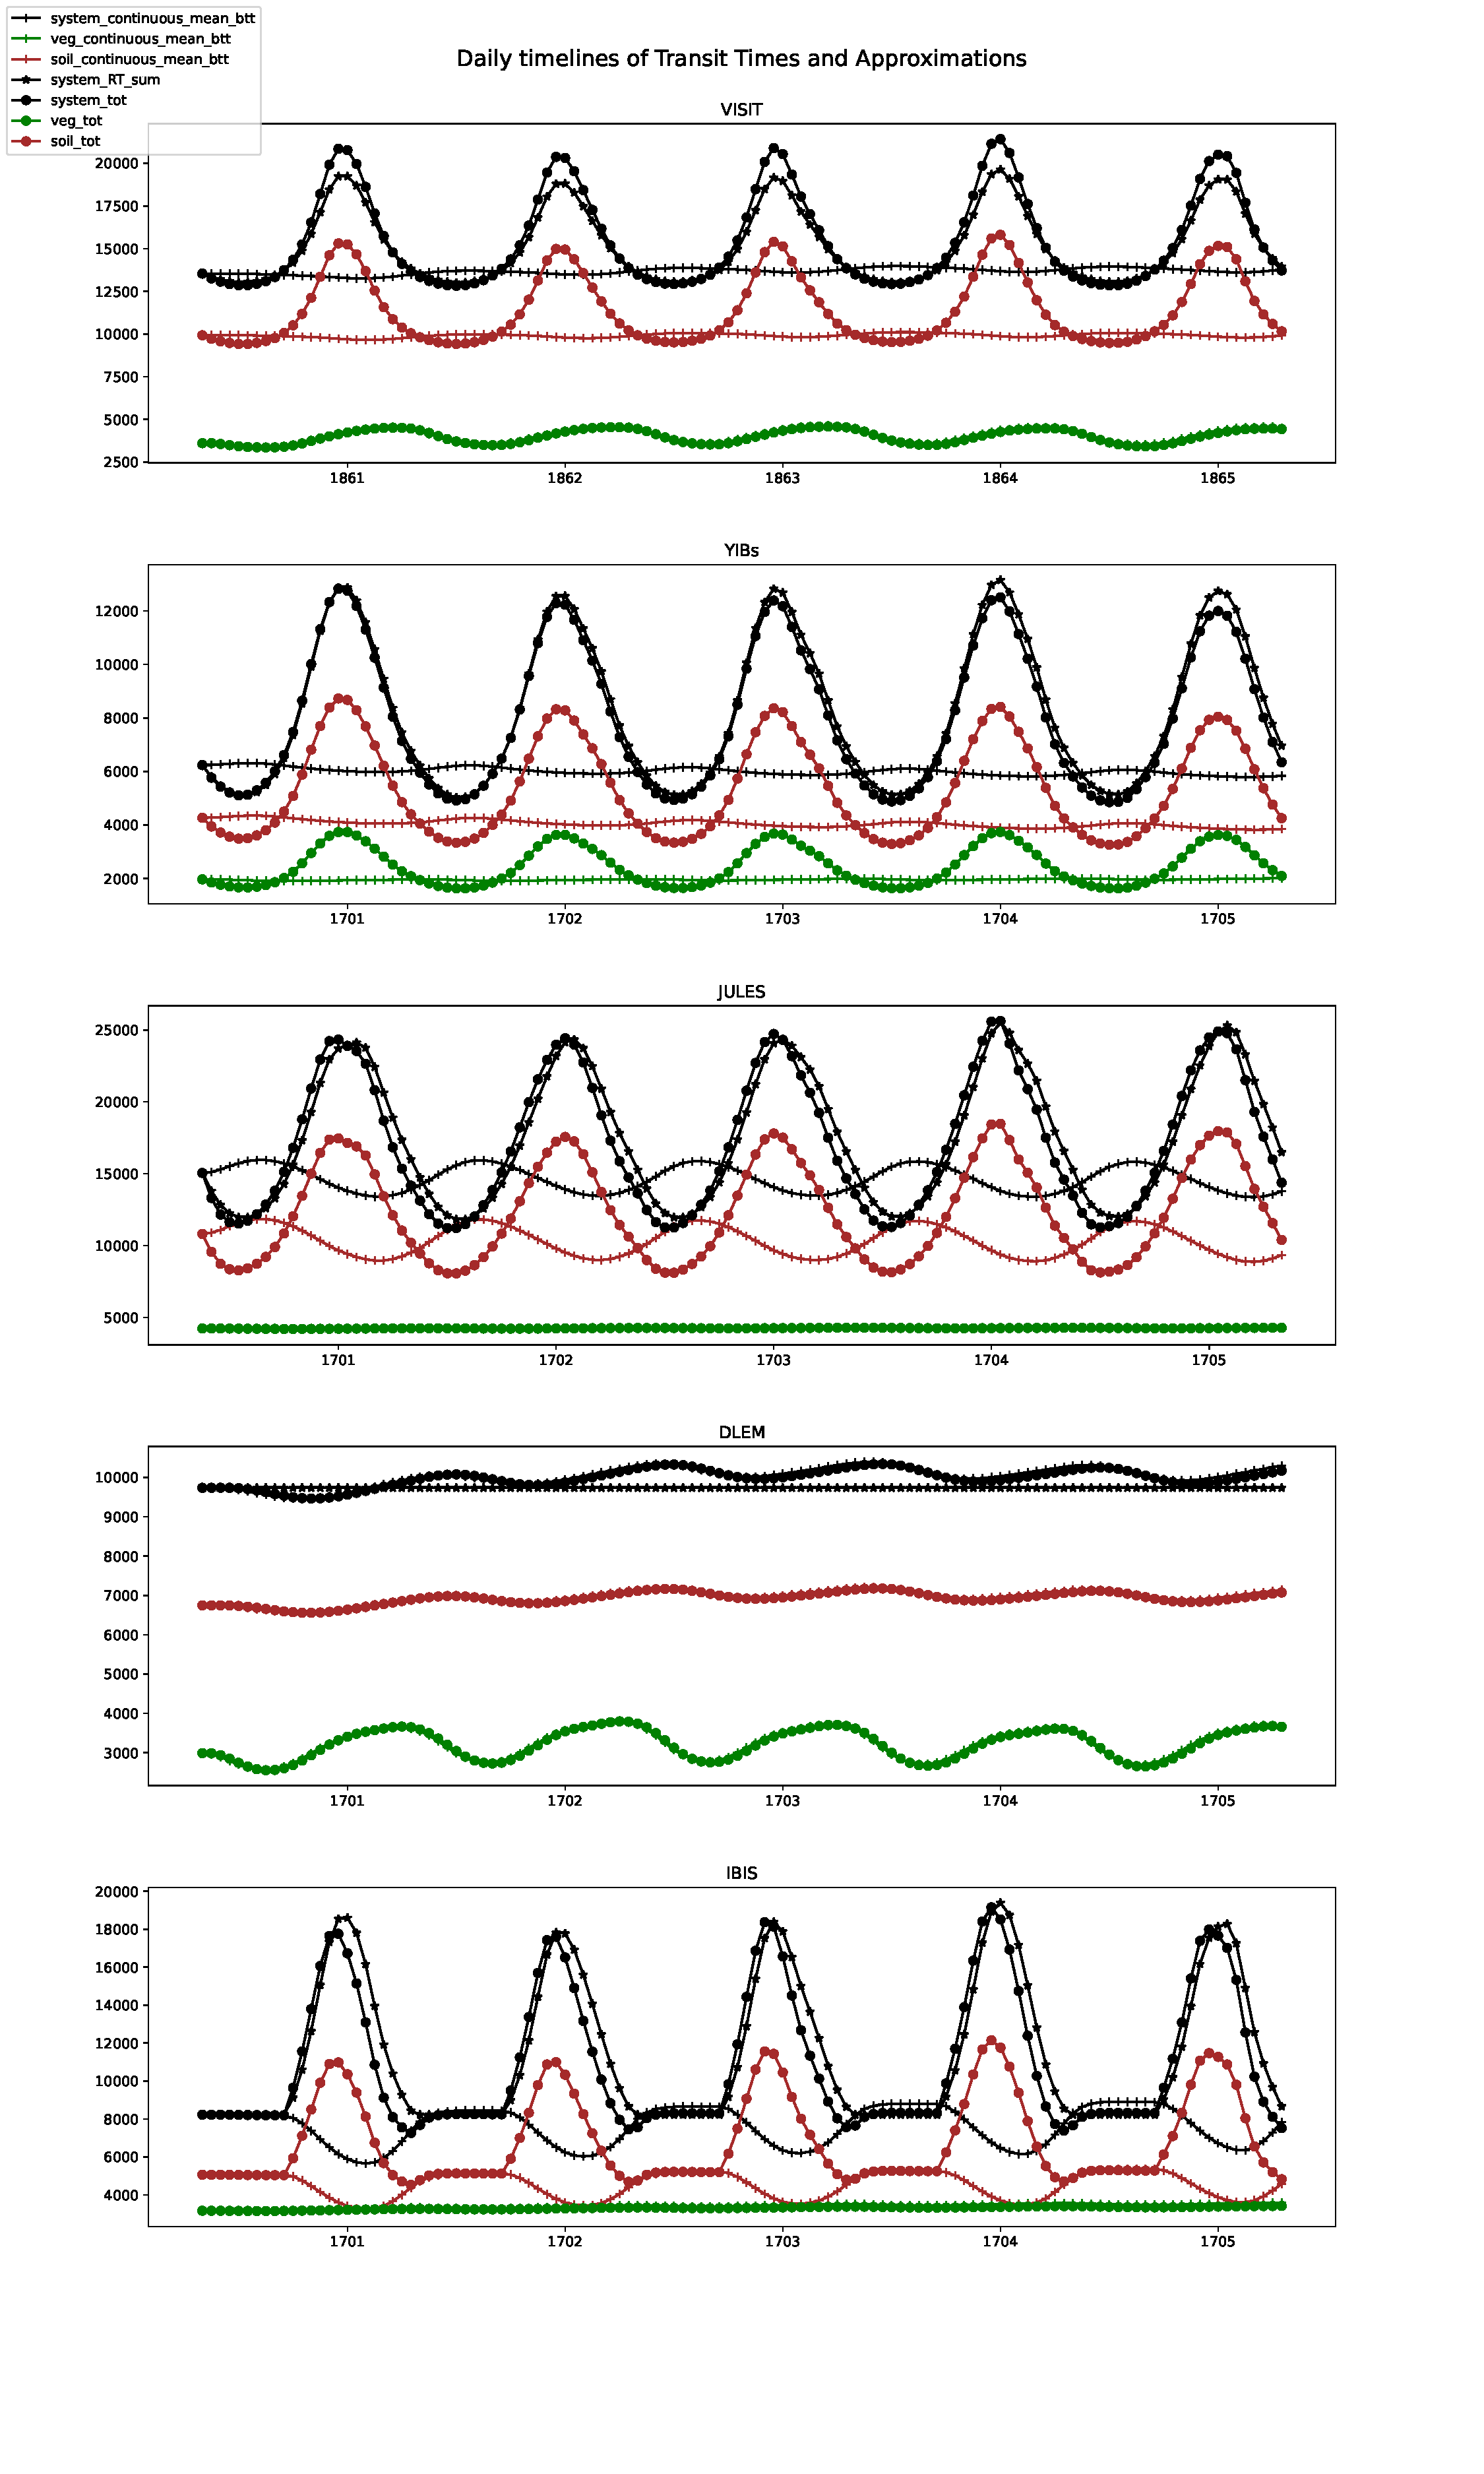
\includegraphics[width=\columnwidth]{test2_fine.pdf}
\end{center}
	%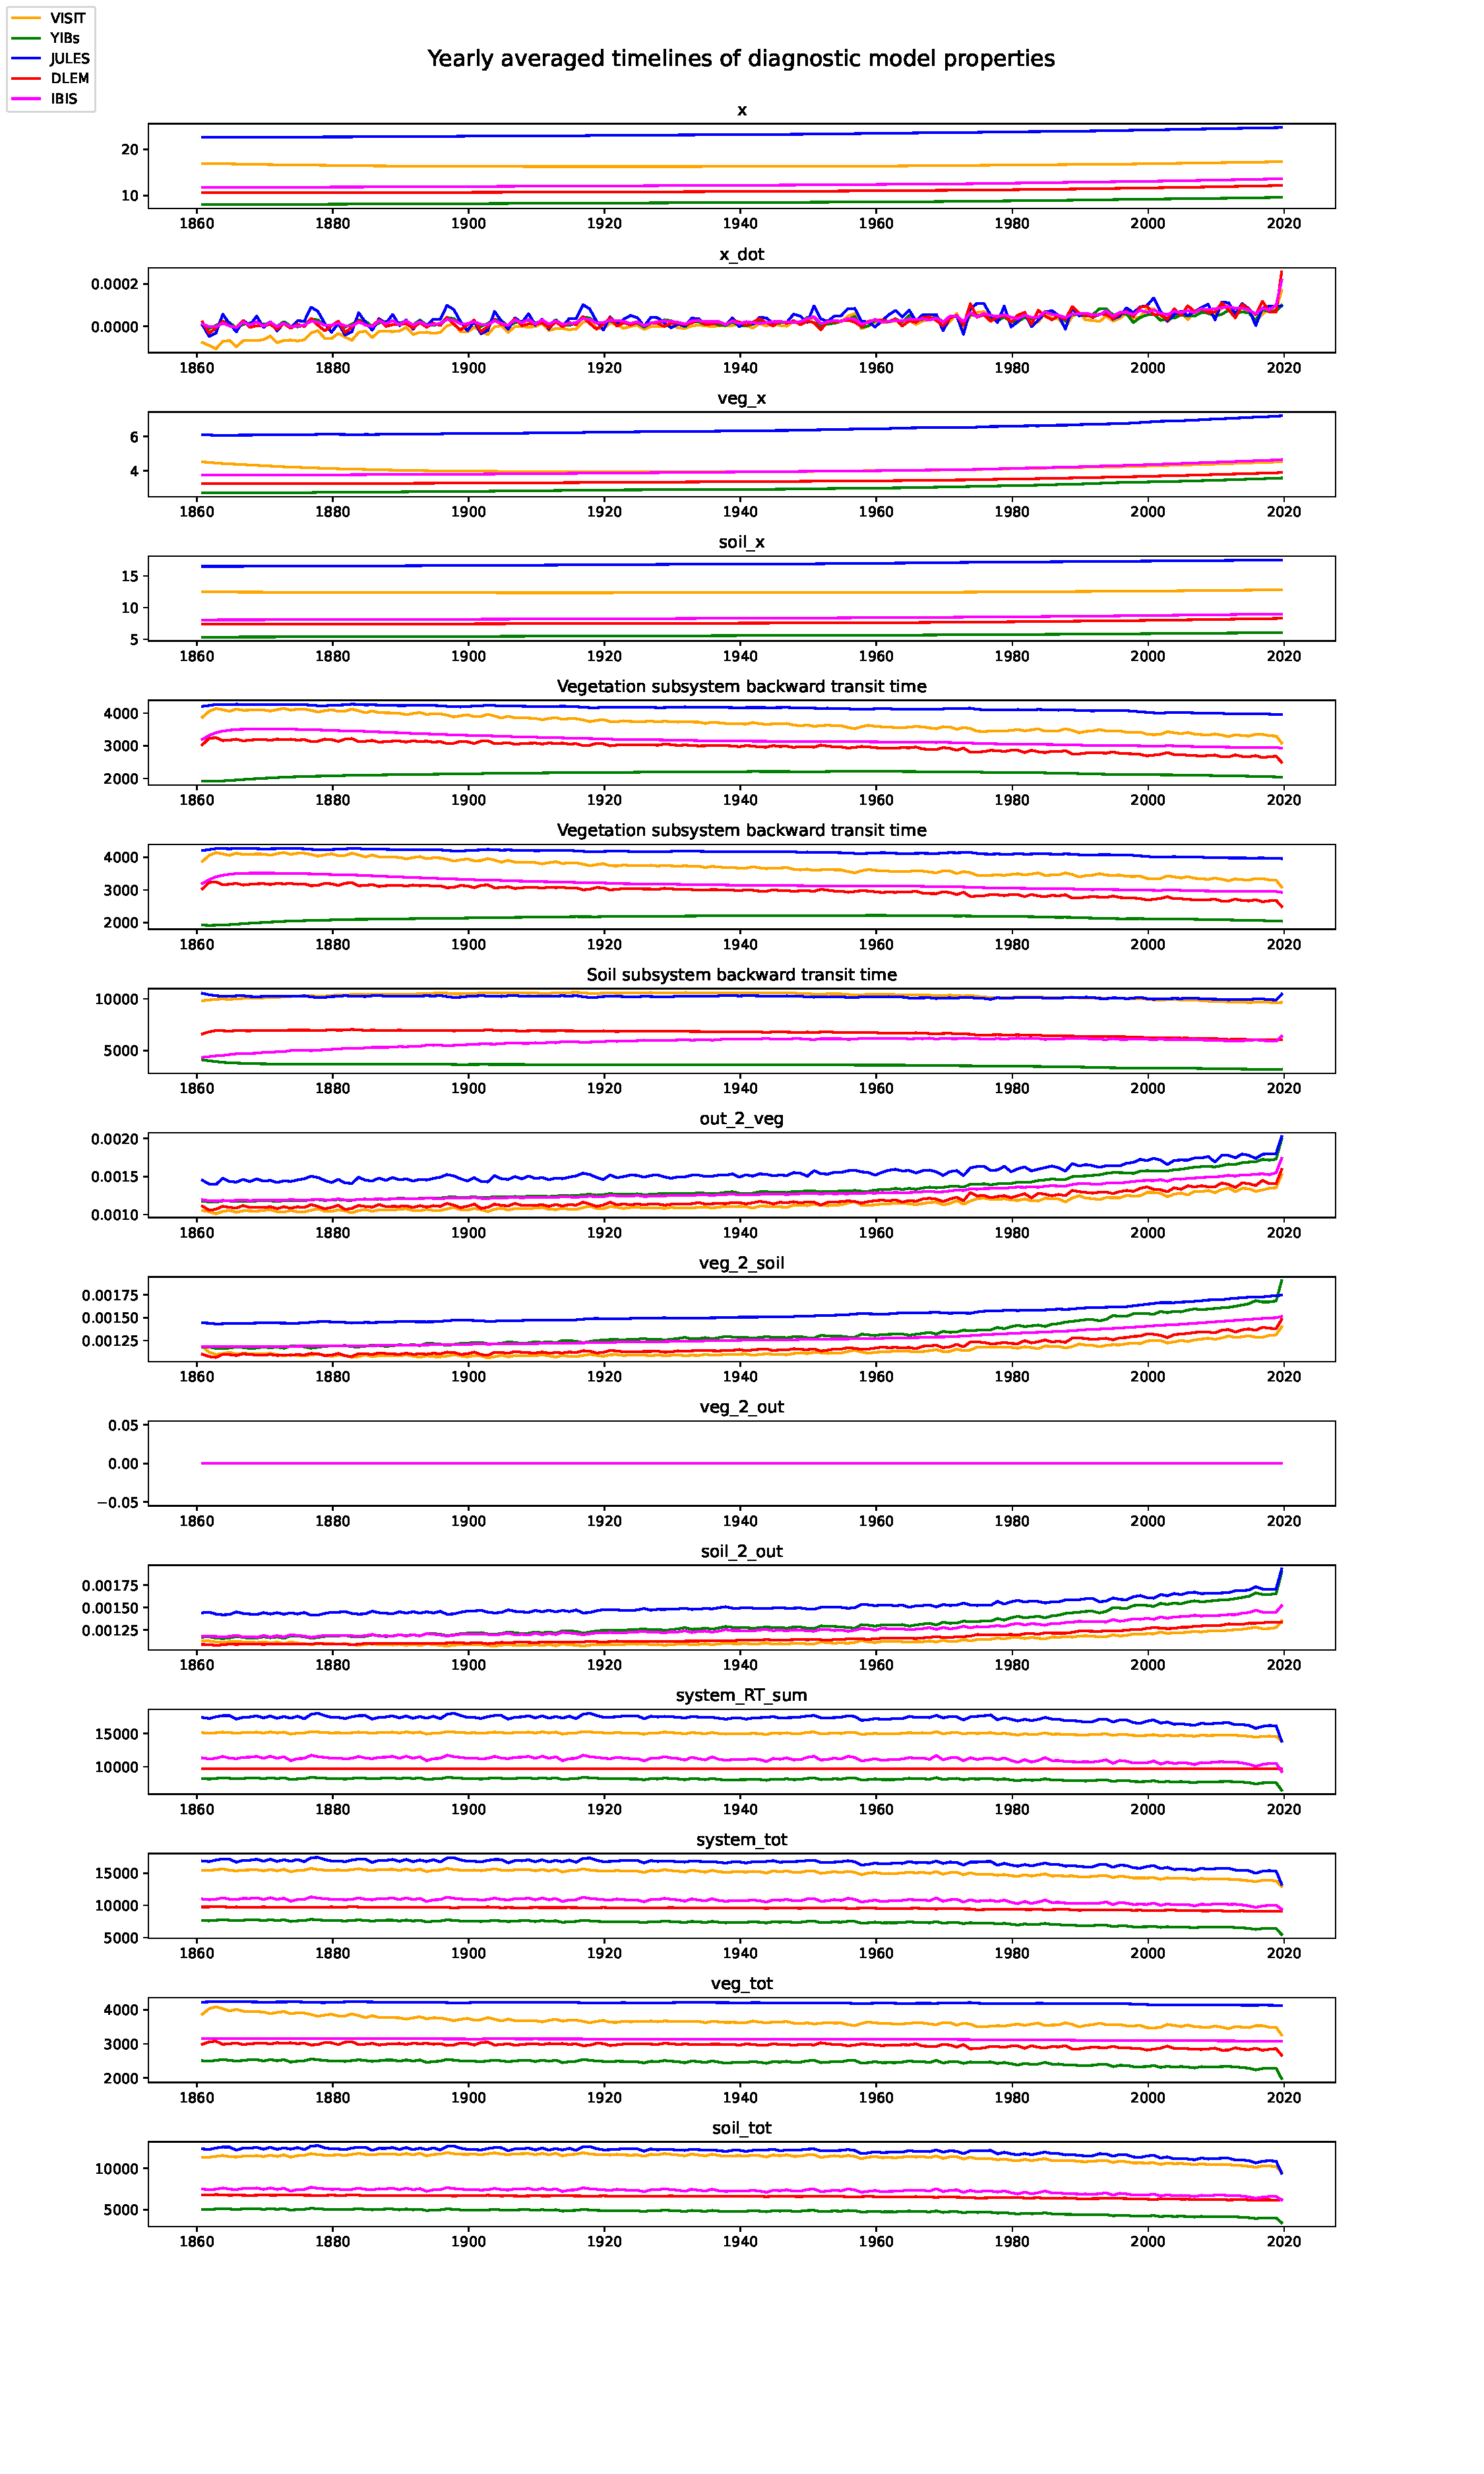
\includegraphics[width=.32\columnwidth]{test_yearly.pdf}
	%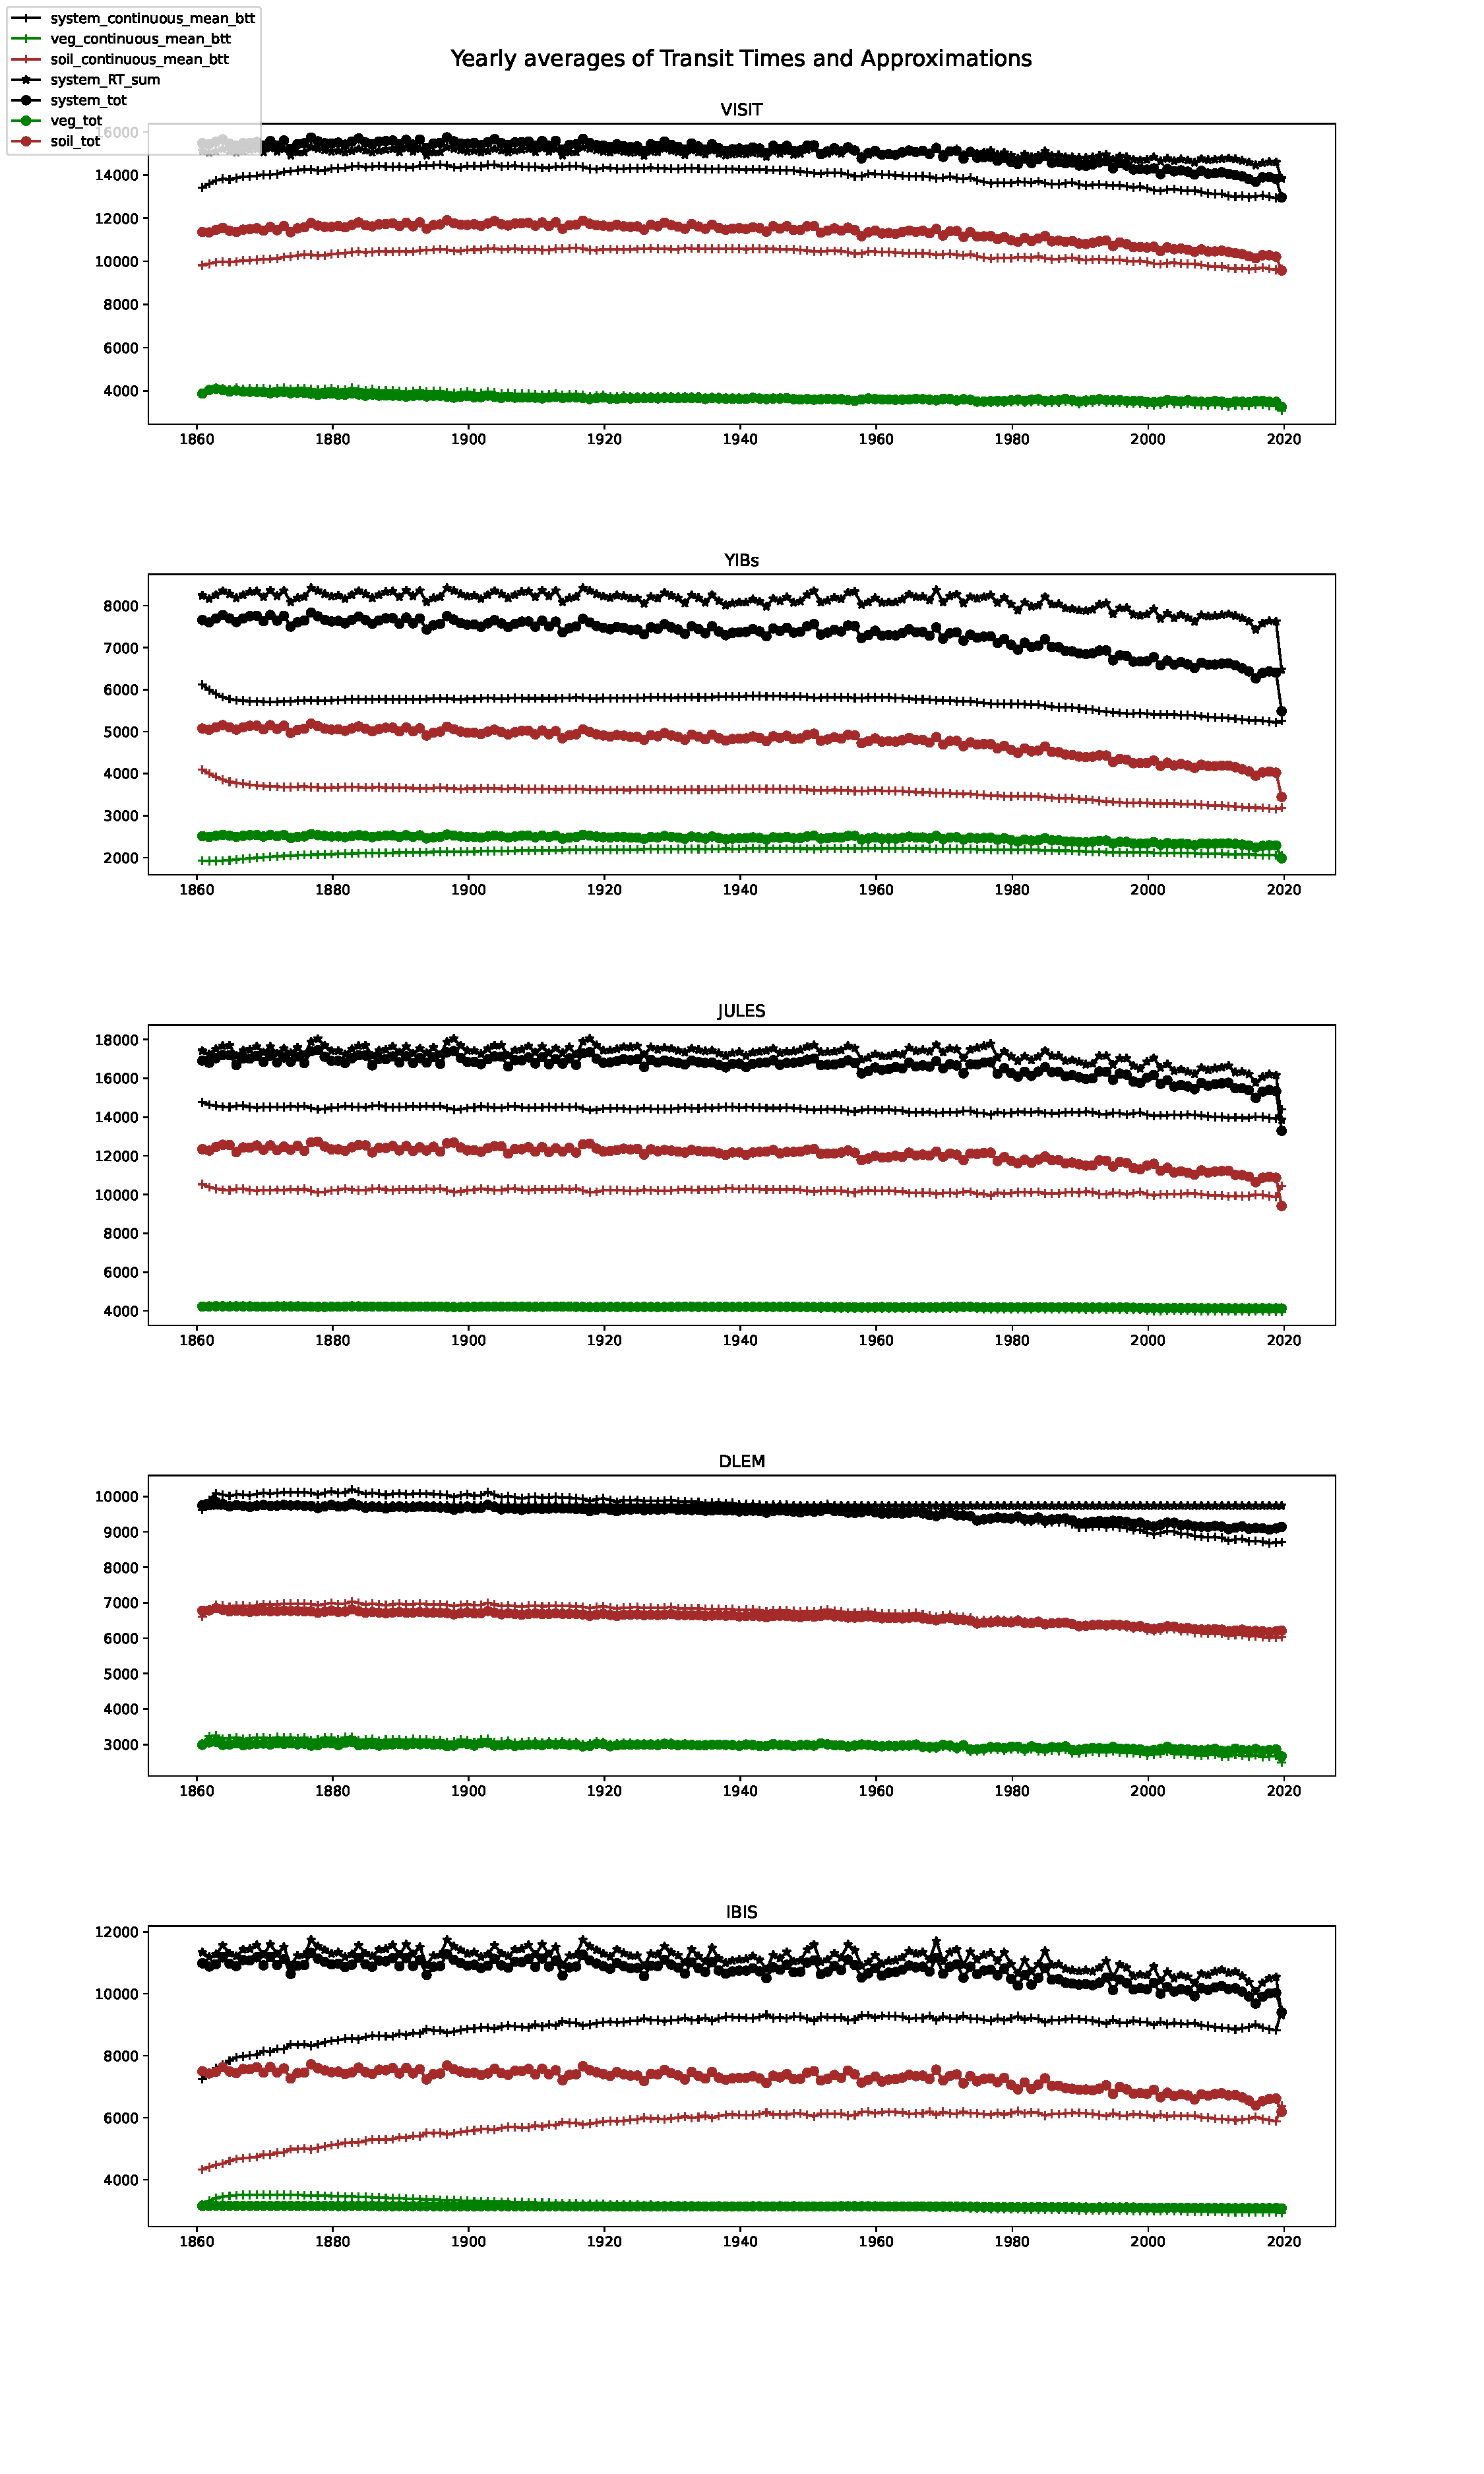
\includegraphics[width=.32\columnwidth]{test2_yearly.pdf}
  %%%%%%%%%%%%%%%%%%%%%%%%%%%%%%%%%%%%%%%%%%%%%%%%%%%%%%%%%%%%%
  \subsubsection*{References}
  \nocite{Luo2017Biogeosciences}
  \nocite{Rasmussen2016JMB}
  \nocite{Metzler2018PNAS}
	%\begin{thebibliography}{}
	%\bibitem[Metzler, Müller, Sierra, 2018]{Metzler2018PNAS}
	%Metzler, H., M{\"u}ller, M., and Sierra, C. (2018).
	%\newblock Transit-time and age distributions for nonlinear time-dependent
	%  compartmental systems.
	%\newblock {\em Proceedings of the National Academy of Sciences}, 115:201705296.
	%\end{thebibliography}
  \tiny{
  \bibliographystyle{abbrvnat}
  \bibliography{TEE-clean.bib}
  }
\end{multicols}


}

%%%%%%%%%%%%%%%%%%%%%%%%%%%%%%%%%%%%%%%%%%%%%%%%%%%%%%%%%%%%%%%%%%%%%%%%%%%%%%%%%%%----
\posterbox[adjusted title=Transparent Source Code]{
  name=code,
  %column*=4,
  column=4,
  %sequence=3 between title and bottom then 4 between top and record
  below=title,
  %column=2,
  %span=1.5,
  %above=bottom
  }{
  
%\section*{Structure} 
\subsubsection*{Integration with python tools }
  %\begin{itemize}
  %\item
   \texttt{bgc\_md2} can be used with all the normal python tools, \texttt{DASK, Jupyter, NumPy, SciPy, SymPy,\dots}
  %\end{itemize}

  %%%%%%%%%%%%%%%%%%%%%%%%%%%%%%%%%%%%%%%%%%%%%%%%%%%%%%%%%%%%%
  \subsubsection*{Sibling \texttt{python} packages}
  \begin{center}
  \begin{tikzpicture}[sibling distance=27em,
    every node/.style = {shape=rectangle, rounded corners,
      draw, align=center,
      top color=white, bottom color=red!20}]
      \node {
      \begin{tikzpicture}[anchor=center]
        \node {
        \texttt{bgc\_md2}
        }
        child { node {\texttt{ComputabilityGraphs}} }
  	    child { node[sibling distance=3em]{\texttt{CompartmentalSystems}}
  	    child { 
          node (LAPM){\texttt{LAPM}}
        }
  	    %child [level distance=3em]{ node (SymPy){\texttt{SymPy}} }
  	    %child [level distance=3em]{ node (NymPy){\texttt{numpy}} }
      };
  	%\draw[->] (LAPM) -- (SymPy); 
    \end{tikzpicture}
    };
  \end{tikzpicture}
  \end{center}

      \texttt{bgc\_md2} is a thin frontend to other \texttt{python} packages. 
      The computability graph computation is outsourced into our package \texttt{ComputabilityGraphs} 
	    Many of the advanced diagnostic variables (age and transittime distributions) are computed using our other packages \texttt{LAPM} and \texttt{CompartmentalSystems} for which \texttt{bgc\_md2} acts as interface.

  %%%%%%%%%%%%%%%%%%%%%%%%%%%%%%%%%%%%%%%%%%%%%%%%%%%%%%%%%%%%%
  \subsubsection*{Internal Structure}
  \begin{center}
  \begin{tikzpicture}[%sibling distance=38em,
    every node/.style = {shape=rectangle, rounded corners,
      draw, align=center,
      top color=white, bottom color=red!20}]]
    \tikzstyle{level 1}=[sibling distance=25.5em]
    \tikzstyle{level 2}=[sibling distance=5em]
    \tikzstyle{level 3}=[sibling distance=3em]
    \tikzstyle{level 4}=[sibling distance=1.75em]
      \node {% <- this 'right of' is inherited; how to avoid?
      \begin{tikzpicture}[anchor=center]
        \node {\texttt{bgc\_md2}
        %\draw (0,0) -- (0,1);
        %\node[fill] at (0,.5) {};
        } 
        child{ node {models}
  	 child{ node{rothC}
  	    child{node {Fluxes}}
  	    child{node {Pools}}
  	    child{node {\dots}}
  	}
        	child{ node {Wang}
  	%    child{node {Fluxes}}
  	%    child{node {Pools}}
  	%    child{node {\dots}}
  	}
        	child{ node {\dots}}
        }
        child{ node {computers}
  	 child{node {Matrix(Fluxes)}}
  	 %child{node {Fluxes(Matrix,Pools)}}
  	 child{node {\dots}}
        };
      \end{tikzpicture}
      };
  \end{tikzpicture}
  \end{center}

    \texttt{bgc\_md2} is not just a collection of models, described as sets of varible of special type like fluxes or matrice, but also 
    a collection of functions whose arguments and return values have these types.
    These functions are here called \texttt{computers} and use python type annotations.
    The computability graph used in the user interface and queries is derived from the 
    annotations of a set of functions.
    The set of properties (defined by the types) can be easily expanded, as well as the functions connecting them.

  %%%%%%%%%%%%%%%%%%%%%%%%%%%%%%%%%%%%%%%%%%%%%%%%%%%%%%%%%%%%%
  \subsubsection*{Database Records are \texttt{python} modules too}
  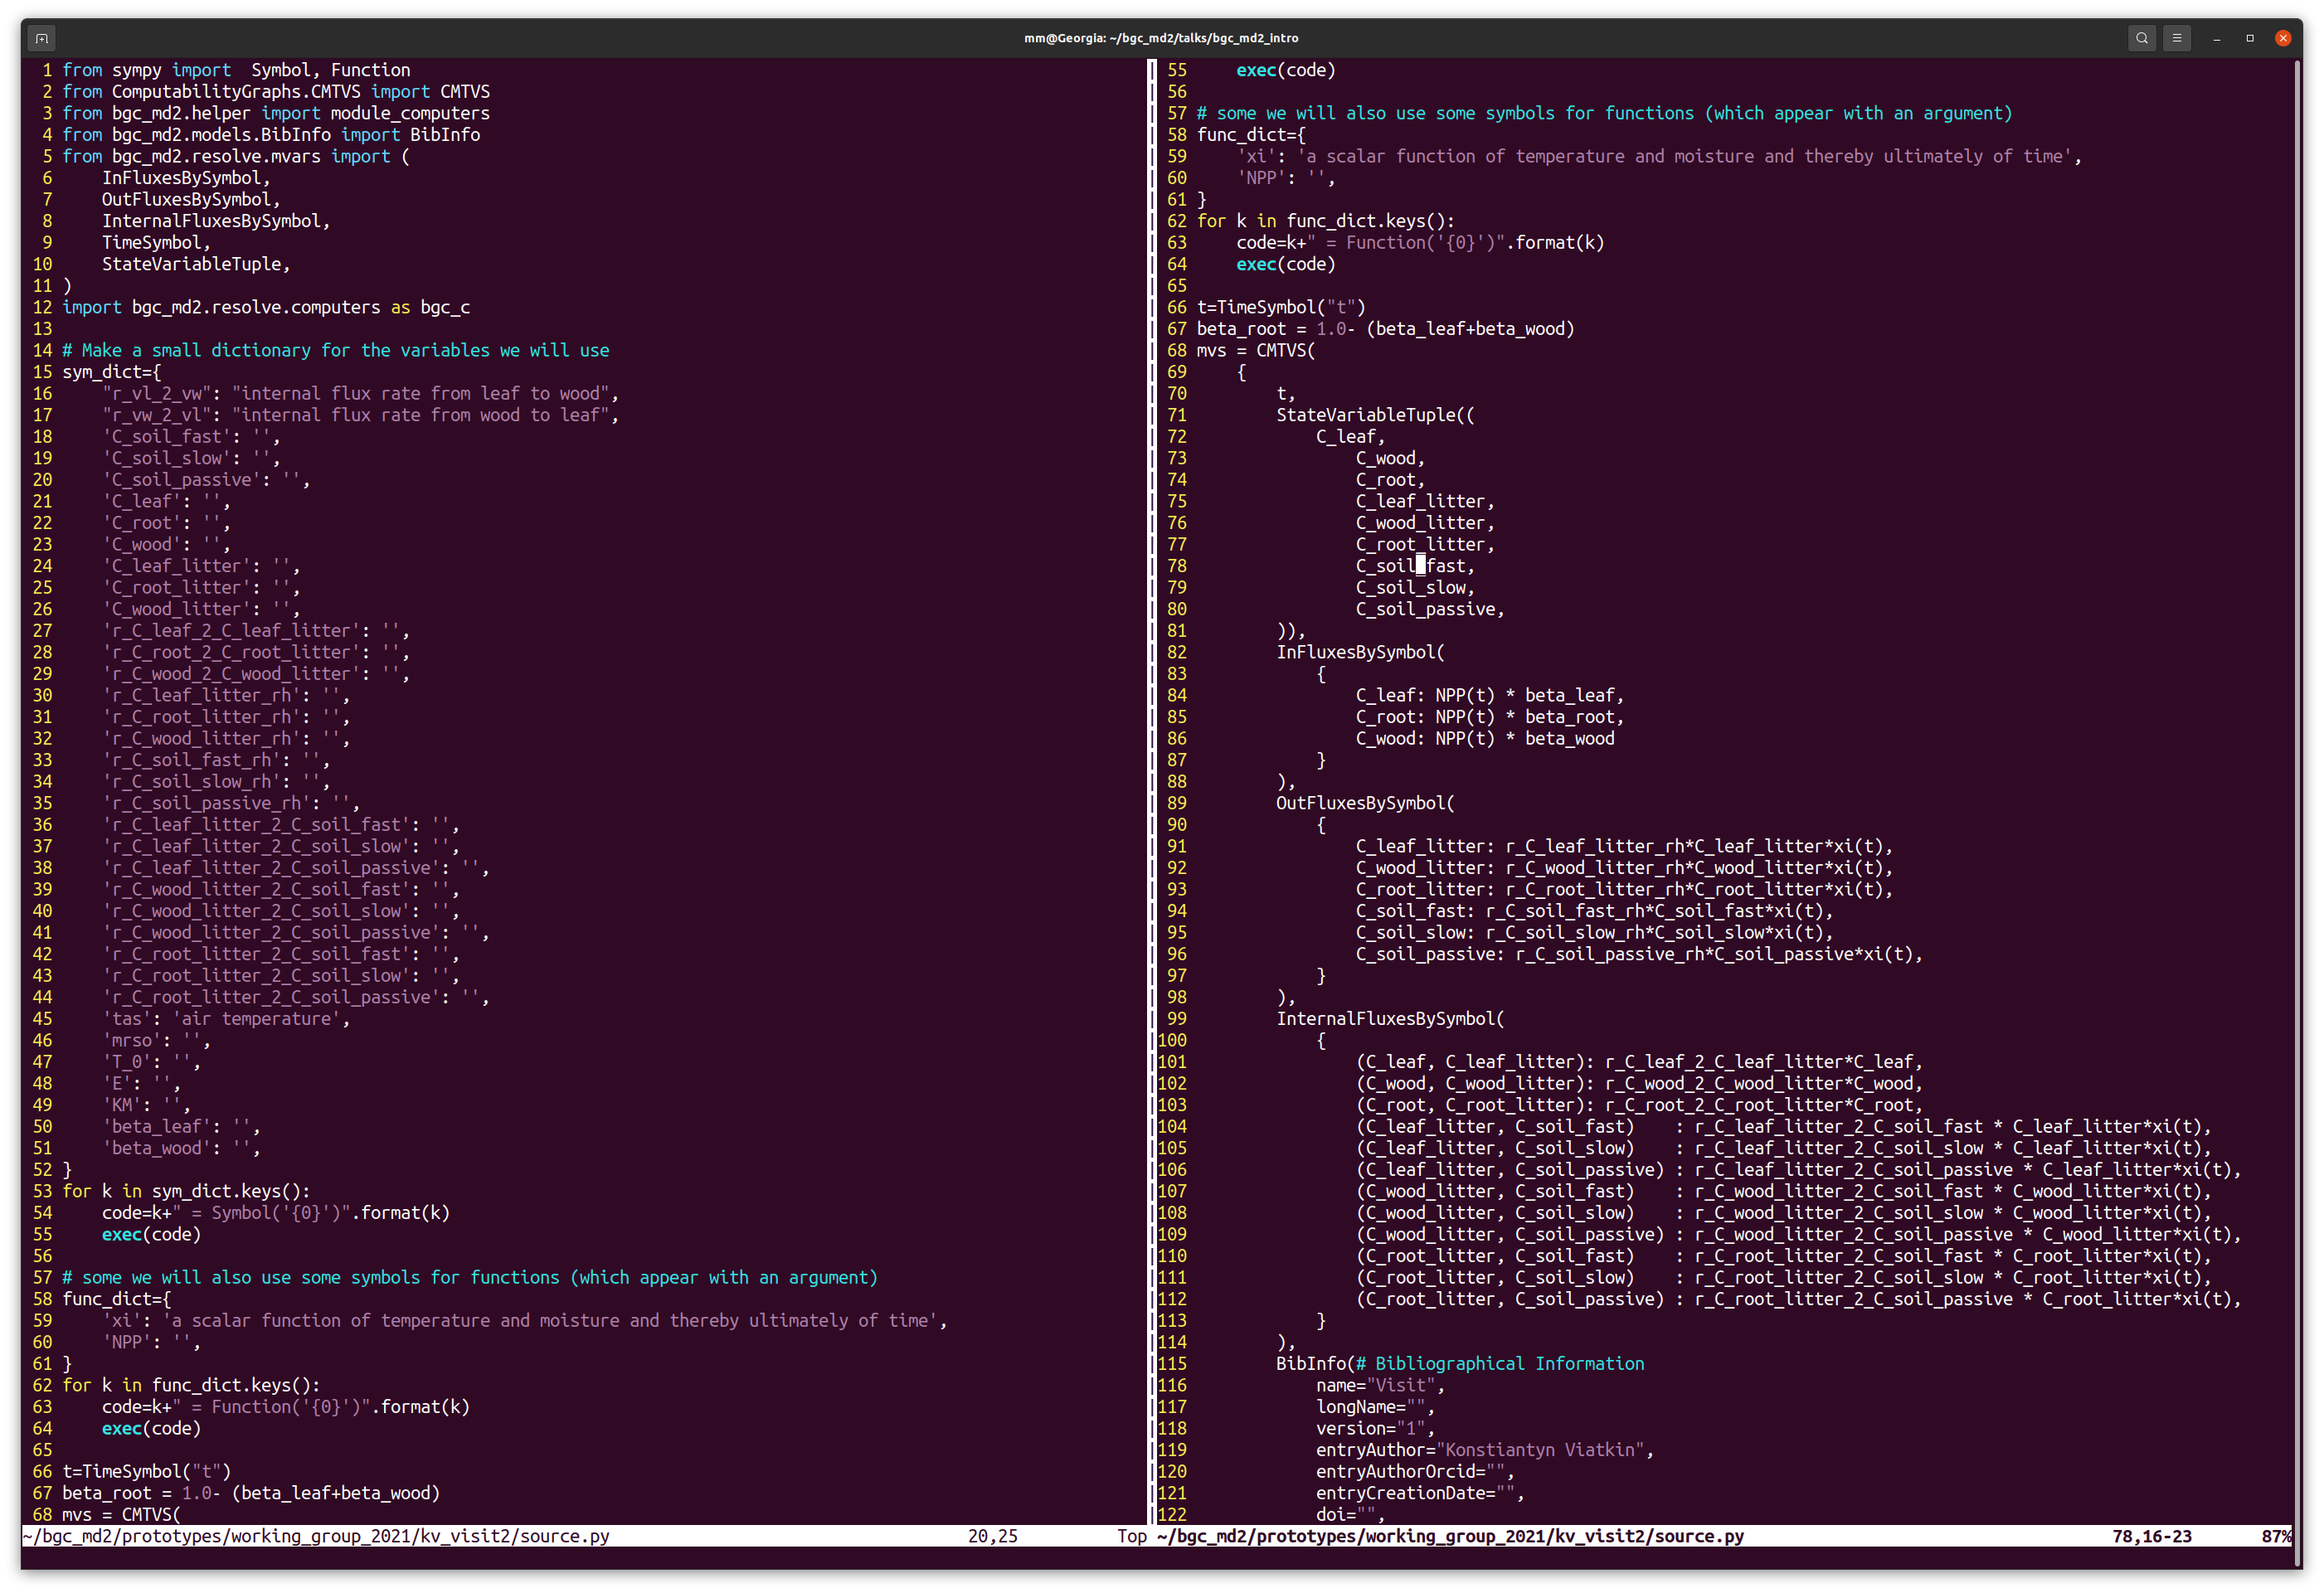
\includegraphics[width=\columnwidth]{source.py.png}
    The picture shows the screen shot of the source code of the above model using sympy and some datatypes provided by \texttt{bgc\_md2}.
    The entries of the database do not have to be complete models. They are implemented in normal python and 
    have in common that they define a set of model properties and a set of functions to connect them.
    wicht are summarized in a \texttt{CMTVS} object (ConnectedMultytypeVariableSet). 
    The creation of all the variables including the the symbolic formulation can be automated by all means available in python.
    Information can but does not have to be provided, and is used to dynamically determine what is computable.

  %%%%%%%%%%%%%%%%%%%%%%%%%%%%%%%%%%%%%%%%%%%%%%%%%%%%%%%%%%%%%
  \subsubsection*{Expandability}
  \texttt{bgc\_md2} and it's sibling packages can acquire new functionality in several ways.
  Ranging from a project defining new models, to full integration by providing new Datatypes and functions
  for the computability graphs.
  
}
%%%%%%%%%%%%%%%%%%%%%%%%%%%%%%%%%%%%%%%%%%%%%%%%%%%%%%%%%%%%%%%%%%%%%%%%%%%%%%%%%%%%%----
%\posterbox[adjusted title=References]{
%  name=references,
%  %column*=4,
%  column=4,
%  below=code
%  %column=2,
%  %span=1.5,
%  %above=bottom
%  }{
%  \nocite{Luo2017Biogeosciences}
%  \nocite{Rasmussen2016JMB}
%  \nocite{Metzler2018PNAS}
%	%\begin{thebibliography}{}
%	%\bibitem[Metzler, Müller, Sierra, 2018]{Metzler2018PNAS}
%	%Metzler, H., M{\"u}ller, M., and Sierra, C. (2018).
%	%\newblock Transit-time and age distributions for nonlinear time-dependent
%	%  compartmental systems.
%	%\newblock {\em Proceedings of the National Academy of Sciences}, 115:201705296.
%	%\end{thebibliography}
%  \tiny{
%  \bibliographystyle{abbrvnat}
%  \bibliography{TEE-clean.bib}
%  }
%}
%%%%%%%%%%%%%%%%%%%%%%%%%%%%%%%%%%%%%%%%%%%%%%%%%%%%%%%%%%%%%%%%%%%%%%%%%%%%%%%%%%%%----
\posterbox[adjusted title=Contact]
    {
    name=contact,
    %column*=4,
    column=4,
    %below=ModelIntercomparison
    %below=references,
    below=code,
    }{
	  \includegraphics[height=5em]{qr_github.pdf}
    \url{https://github.com/MPIBGC-TEE/bgc\_md2\#readme}
    \\
	  \includegraphics[height=5em]{qr_mm.pdf}
    \url{mailto:markus.mueller.1.g@googlemail.com}
}
\end{tcbposter}
\end{document}

